\documentclass{article}
\usepackage[utf8]{inputenc}
\usepackage[spanish]{babel}
\usepackage{graphicx}	%Si se quiere compilar con las imagenes
% \usepackage[draft]{graphicx}	%Si NO se quiere compilar con las imagenes porque tarda mucho
\usepackage{graphics, float, fancyhdr, titling, caption, subcaption}
\usepackage{listings, xcolor}
\usepackage[a4paper, total={6in, 9.5in}]{geometry}
\usepackage{fancyhdr}
\usepackage{hyperref}		% solo se debe usar si se quiere usar \hypersetup
\usepackage{xurl}


% \usepackage{amsmath}      % Si se quiere usar \text{texto} dentro del modo matematico
%\setcounter{secnumdepth}{-2}       %Poner solo esto si no se quieren numero delante de las secciones y niveles inferiores.

\renewcommand{\footrulewidth}{0.4pt}
\title{

\includegraphics[width=1.75in]{imagenes/UGR-Logo.png} \\
\vspace*{1in}
\textbf{Cuestiones Tema 4} \\
Animación por Ordenador \\
\vspace*{0.5in}}
\author{Andrés Merlo Trujillo \\
andresmerlo@correo.ugr.es \\
77147239H \\ 
\vspace*{0.5in} \\
E.T.S. de Ingenierías Informática y de Telecomunicación \\
\textbf{Universidad de Granada}} \date{\today}

\hypersetup{
    colorlinks=true,
    linkcolor=black,
    citecolor=black
}

\renewcommand\maketitlehooka{\null\mbox{}\vfill}
\renewcommand\maketitlehookd{\vfill\null}

\definecolor{codegreen}{rgb}{0,0.6,0}
\definecolor{codegray}{rgb}{0.5,0.5,0.5}
\definecolor{codepurple}{rgb}{0.58,0,0.82}
\definecolor{backcolour}{rgb}{0.95,0.95,0.92}

\lstdefinestyle{mystyle}{
    backgroundcolor=\color{backcolour},   
    commentstyle=\color{codegreen},
    keywordstyle=\color{magenta},
    numberstyle=\tiny\color{codegray},
    stringstyle=\color{codepurple},
    basicstyle=\ttfamily\footnotesize,
    breakatwhitespace=false,         
    breaklines=true,                 
    captionpos=b,                    
    keepspaces=true,                 
    numbers=left,                    
    numbersep=5pt,                  
    showspaces=false,                
    showstringspaces=false,
    showtabs=false,                  
    tabsize=2
}

\lstset{style=mystyle}

\lstdefinelanguage{MaxScript}{
  keywords={break, case, catch, collect, continue, coordsys, default, do, else, exit, false, for, fn, global, if, in, local, macroScript, not, of, on, plugin, return, rollouts, silent, struct, then, to, true, try, undo, utilities, when, while, quat, rotate},
  keywordstyle=\color{blue}\bfseries,
%   ndkeywords={!=, #, #_, ##, %, &amp;, \&, \&, *, **, +, -, /, //, :, &lt;&lt;, &gt;&gt;, &lt;=, &gt;=, ==, ^, ~, ~=, +=, -=, *=, /=, //=, ^=, &=, &lt;&lt;=, &gt;&gt;=},
%   ndkeywordstyle=\color{red}\bfseries,
  identifierstyle=\color{black},
  sensitive=true,
  comment=[l]{--},
  morecomment=[s]{/*}{*/},
  commentstyle=\color{codegreen}\ttfamily,
  stringstyle=\color{purple}\ttfamily,
  morestring=[b]',
  morestring=[b]"
}


\begin{document}
\begin{titlingpage}
\maketitle
\end{titlingpage}

\tableofcontents

\newpage

\pagestyle{fancy}   %a partir de comienza el header (se salta el indice y portada)
\fancyhead[L]{Andrés Merlo Trujillo}
\fancyhead[R]{Animación por Ordenador}
%\section{Ejercicio 1}
%\begin{figure}[H]
%    \centering
%    \includegraphics[width=\textwidth]{imagenes/passwdfile.png}
%    \vspace{10pt}
%    \footnotesize{Fuente: https://...}
%\end{figure}

% \begin{figure}[H]\ContinuedFloat		% si se parten las imagenes en dos paginas y se desea continuar las letras de las subfiguras (a, b, c, ..., otra pag -> c, d, e)
% \begin{figure}[H]
%     \centering 
% 	\begin{subfigure}[t]{0.48\textwidth}
% 	    \centering
% 	    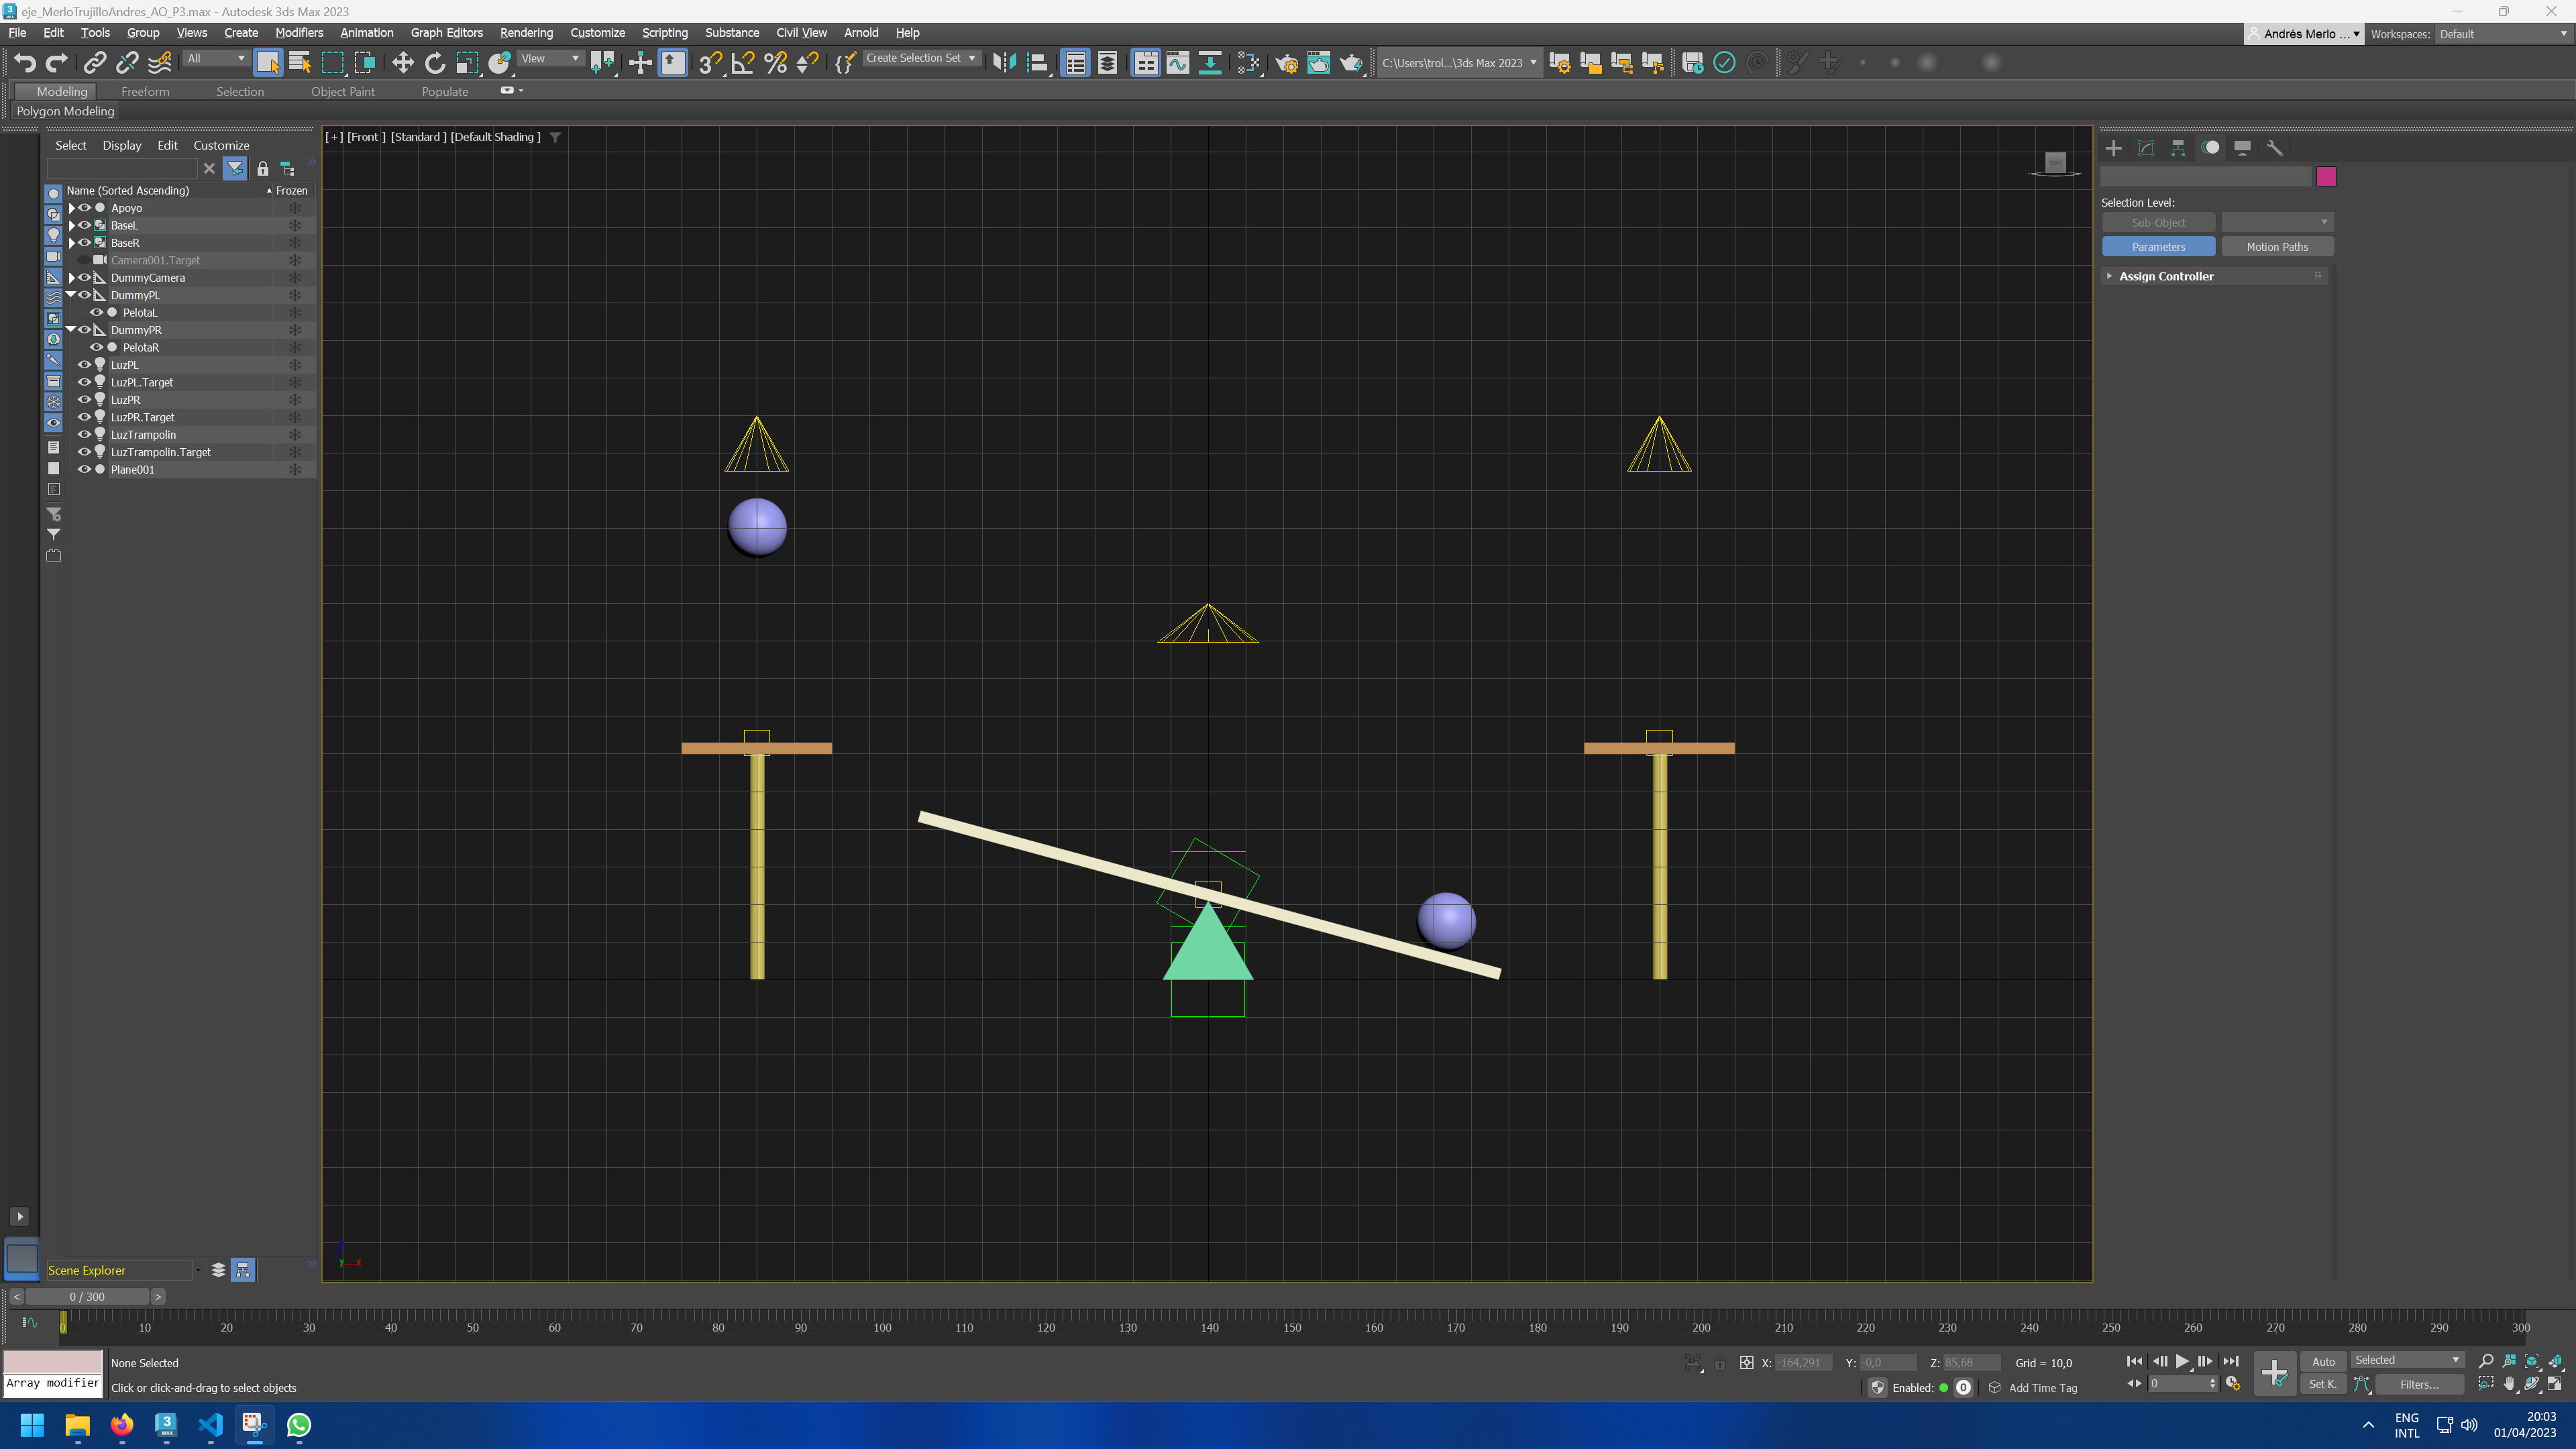
\includegraphics[width=\textwidth]{imagenes/Ejercicio 1/keyframes/0.png}
%         \caption{Pelotas en el instante 0.}
%     \end{subfigure}
%     \hfill
%     %\par\bigskip %si se desea dejar un margen entre la imagen de arriba y de abajo
% 	\begin{subfigure}[t]{0.48\textwidth}
% 	    \centering
% 	    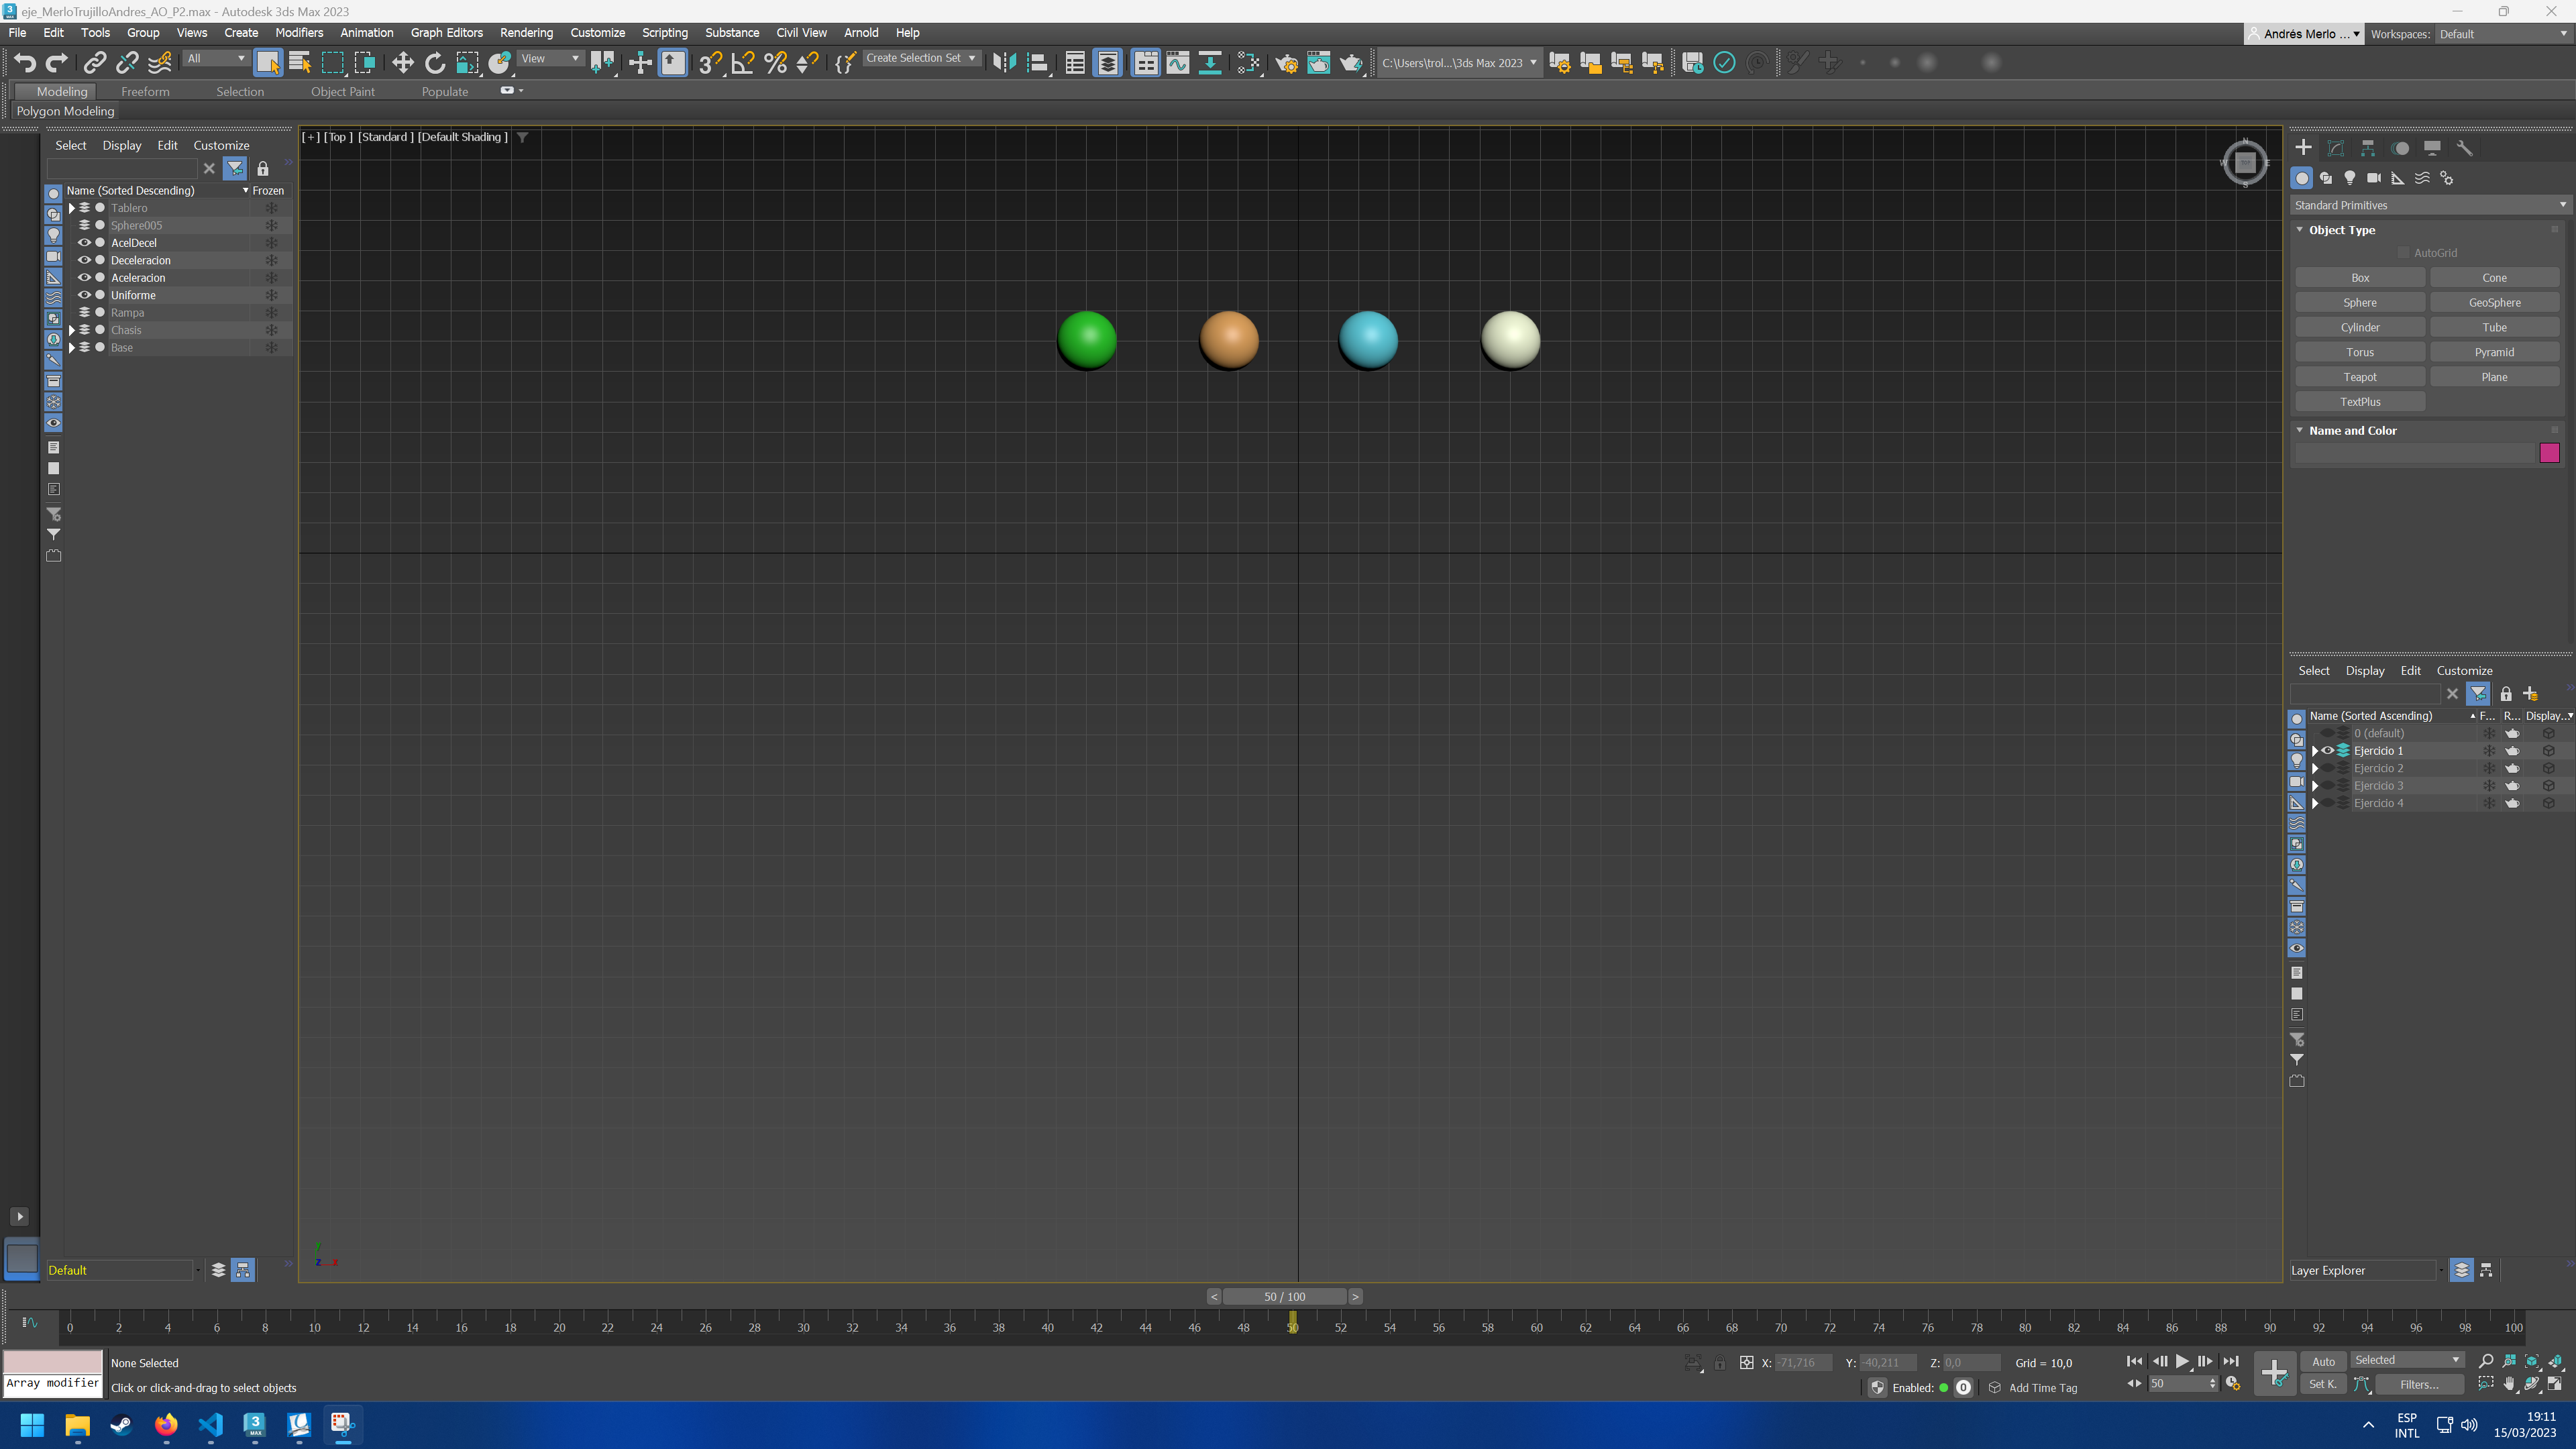
\includegraphics[width=\textwidth]{imagenes/Ejercicio 1/keyframes/50.png}
%         \caption{Pelotas en el instante 50.}
%     \end{subfigure}    
% \end{figure}

% $30 \text{fps} \times 2 \times 5 \text{segundos} = 300 \text{fotogramas} $

\section{Localiza en 3DS Max estos canales e indica qué serían cada uno de ellos.}

Los canales en 3DS Max se pueden ver en el editor de curvas, con un objeto seleccionado. Además, estos canales dependen de la animación que se haya hecho para dicho objeto, por lo que puede ser variable. 

% foto de un cubo
\begin{figure}[H]
    \centering
    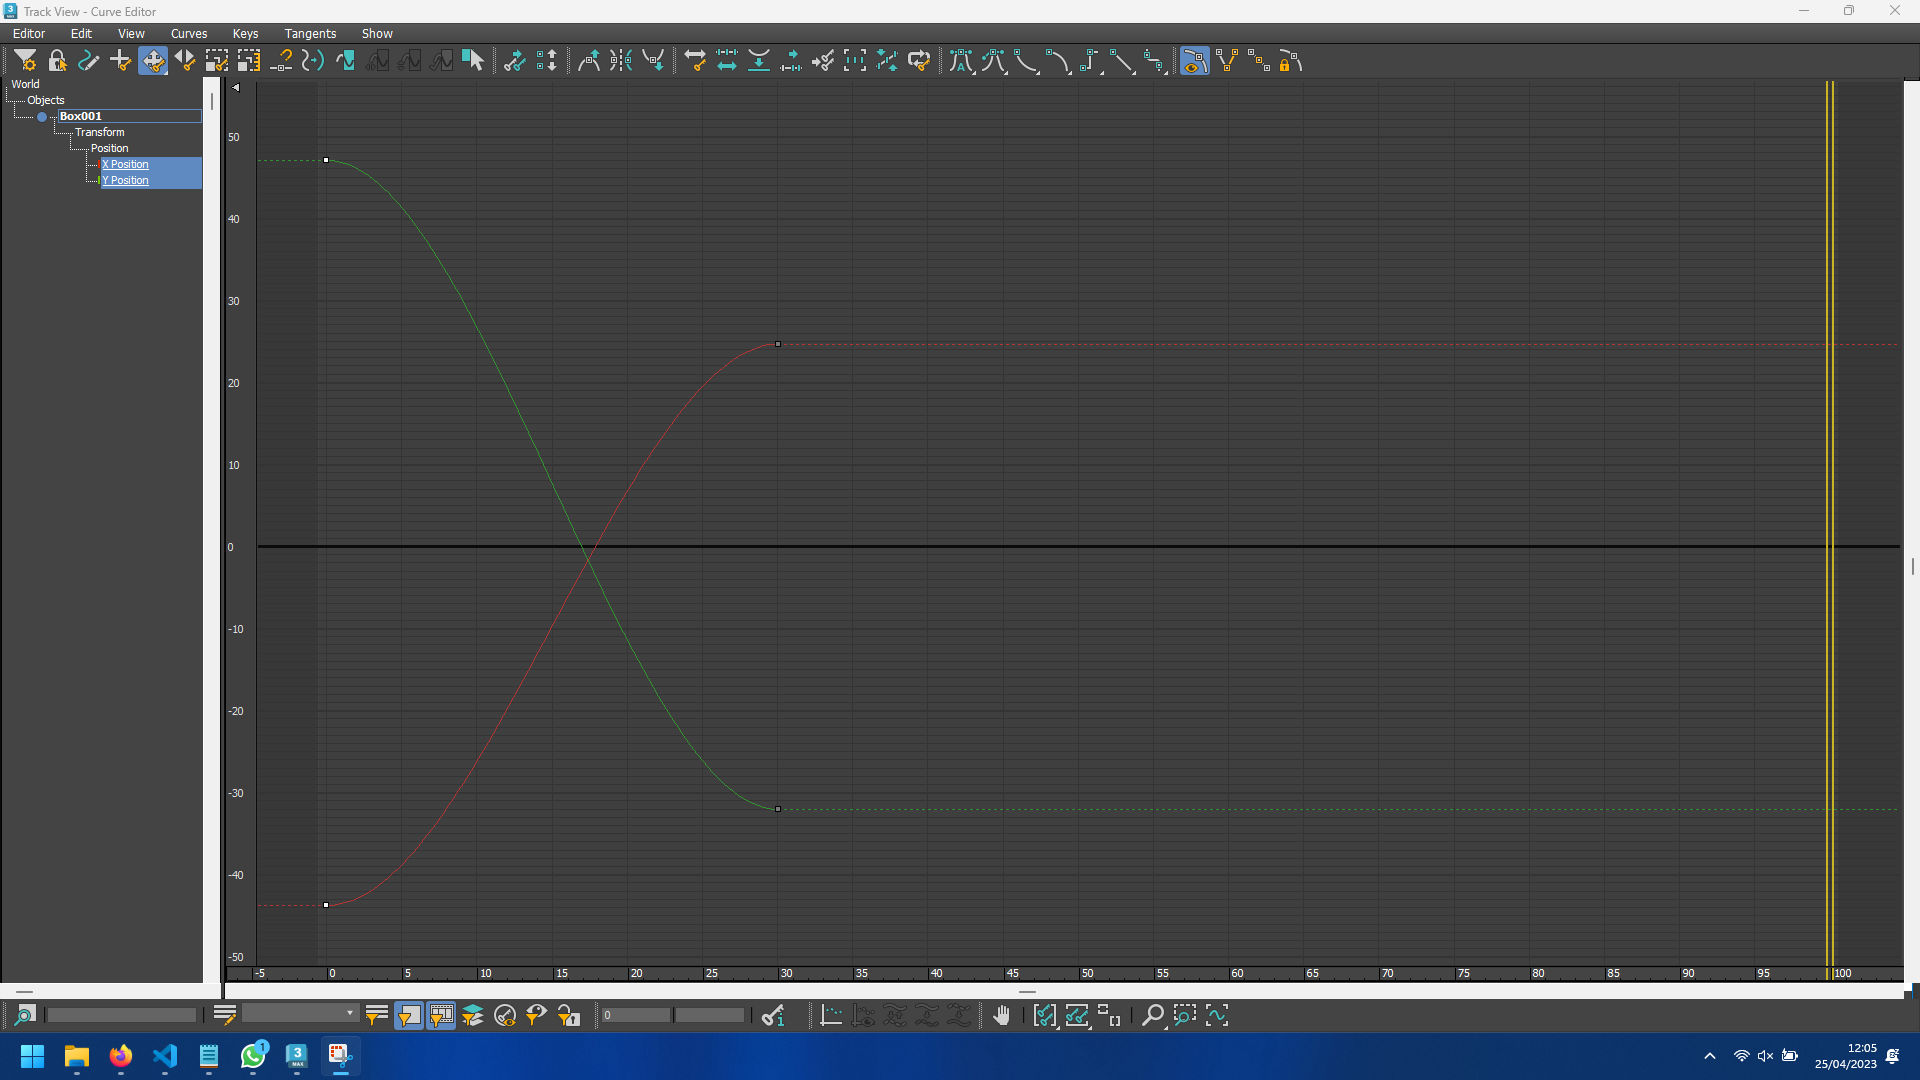
\includegraphics[width=0.7\textwidth]{imagenes/11.png}
    \caption{Canales del cubo.}
\end{figure}

En el caso del cubo, se puede ver que tiene dos canales: el de posición en el eje X y el de posición en el eje Y \cite{explicacion}.

\begin{figure}[H]
    \centering
    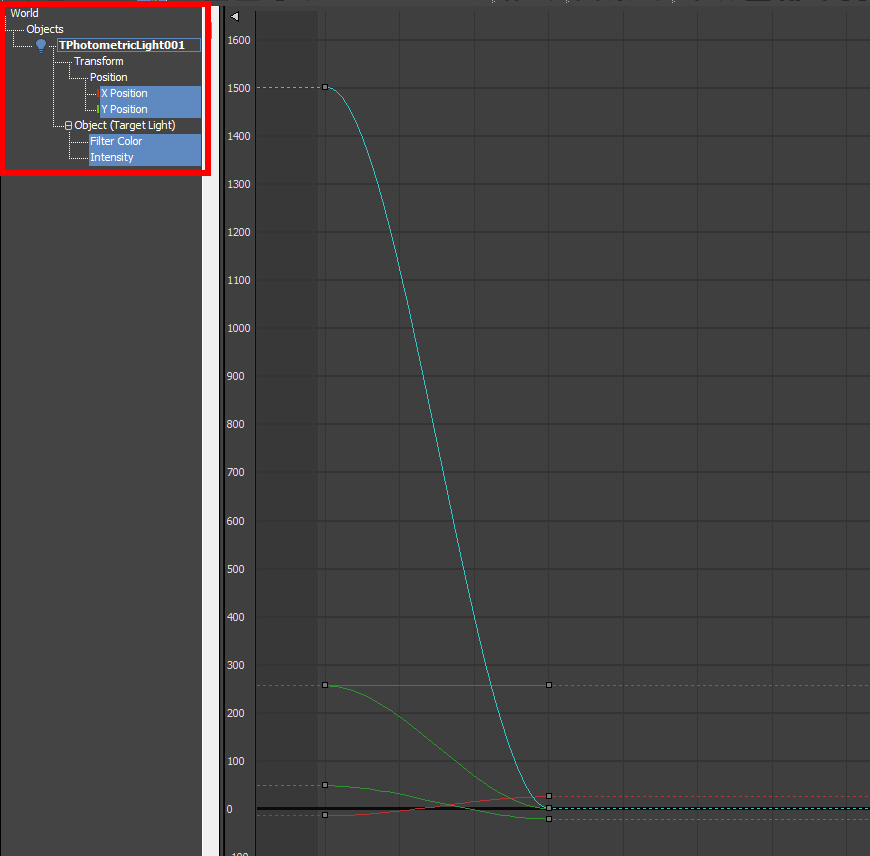
\includegraphics[width=0.7\textwidth]{imagenes/12.png}
    \caption{Canales del \textit{Target Light}.}
\end{figure}

En este caso, la luz tiene 4 canales: los mismos que el cubo para la posición en el eje X e Y, el color de la luz y su intensidad \cite{explicacion}.

\bigskip

Por tanto, se puede decir que el número de canales viene determinado por cada ``curva'' que tenga el objeto asociado; es decir, por el número de atributos que se anime en el objeto.


% mejorar
\section{Indica las ventajas e inconvenientes trabajando con poses frente a canales.}

Ventajas de trabajar con poses: 

\begin{itemize}
    \item Más rápido a la hora de reproducir animaciones, ya que el vector indica directamente las propiedades del objeto en un momento dado.
    \item Almacenamiento contiguo en memoria, lo que permite un acceso más rápido por parte del procesador.
\end{itemize}

\bigskip

Mientras que las desventajas de utilizar poses son:

\begin{itemize}
    \item Dificultad para añadir o eliminar canales, al ser necesario modificar la estructura del vector en todos los instantes.
\end{itemize}

\bigskip
\newpage

Si bien solo se pedían las ventajas y desventajas de usar poses frente a canales, he preferido indicar las ventajas y desventajas de los canales frente a poses también. Por tanto, las ventajas de usar canales son:

\begin{itemize}
    \item Posibilidad de optimizar el almacenamiento de la estructura de datos, al ser independientes una de otras.
    \item Independencia entre canales, permitiendo añadir o eliminar nuevos canales de forma rápida y directa.
\end{itemize}

\bigskip

Mientras que las desventajas son:

\begin{itemize}
    \item Necesidad de evaluar de forma independiente cada canal para saber que atributos tiene la escena en un momento dado. Esto implica acceso a cada canal, que no está en memoria de forma contigua, haciendo que se requiera tiempo y cómputo adicional \cite{diapos}.
\end{itemize}

\section{¿Qué tipo de interpolación hace por defecto 3DS Max entre dos fotogramas clave definidos manualmente en términos de \textit{spacing}?}

Para saber que tipo de \textit{spacing} se utiliza, es necesario animar un objeto para que se mueva de un lado a otro y después ver su \textit{Motion Path} \cite{explicacion}.

% Foto de la animacion
\begin{figure}[H]
    \centering
    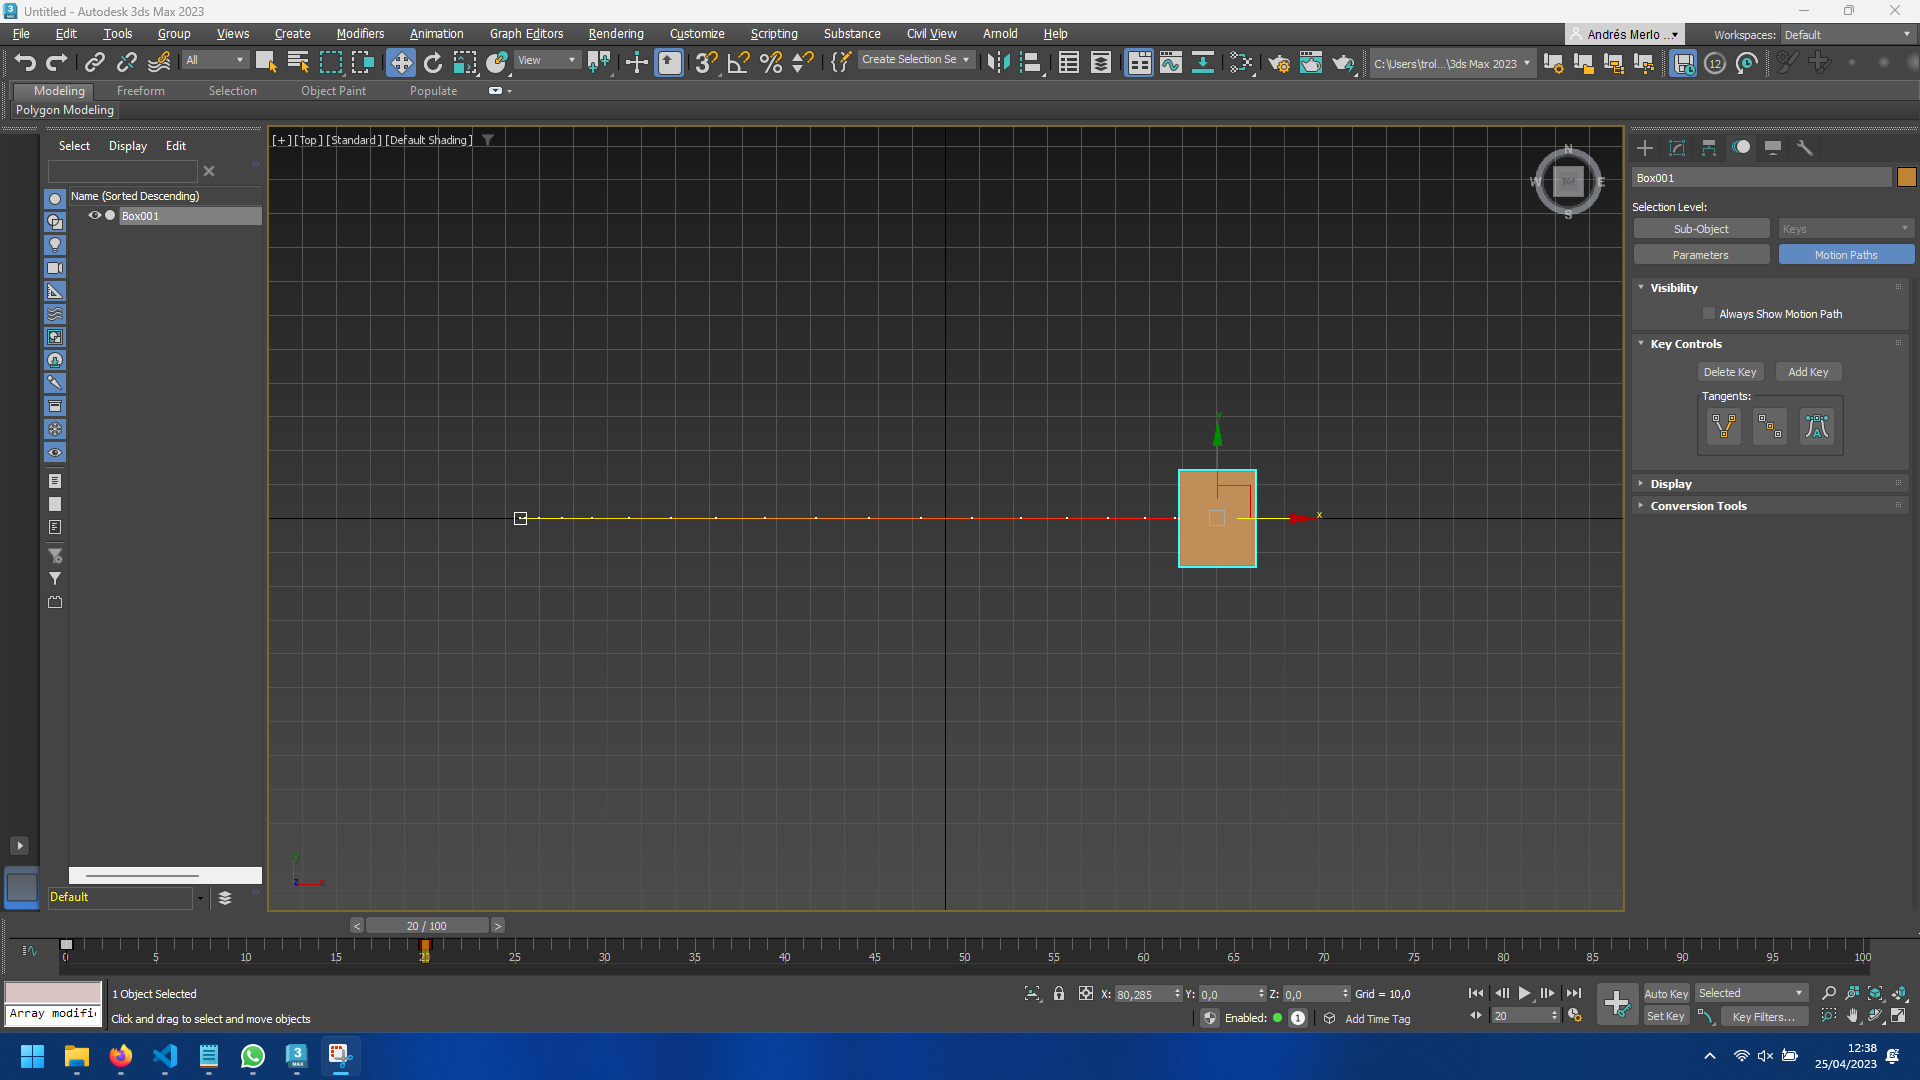
\includegraphics[width=0.8\textwidth]{imagenes/3-1.png}
    \caption{\textit{Motion Path} seguido por un cubo animado.}
\end{figure}

% Como se puede ver, el número de puntos es mayor y más cercanos en los bordes que en el centro, dando a entender de que se sigue un espaciado no lineal.
Como se puede ver, sigue una línea recta, dando a entender que sigue una interpolación línea. No obstante, también se puede ver que el número de puntos es mayor en los bordes y menor en el centro, por lo que es no uniforme. 


% escribir sobre mas puntos

\newpage
\section{¿Qué información almacena un fotograma clave?}

Para ver que información almacena un fotograma clave en 3DS Max, es necesario animar un objeto e irse al editor de curvas. A continuación, es necesario seleccionar un punto de cualquier curva y darle clic derecho \cite{explicacion}.

\bigskip

Aparecerá la siguiente ventana:

% foto de la ventana
\begin{figure}[H]
    \centering
    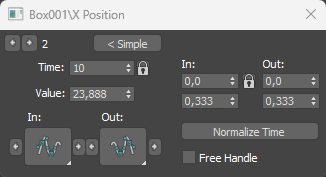
\includegraphics[width=0.6\textwidth]{imagenes/4-1.png}
    \caption{Ventana con los datos que almacena para cada fotograma clave.}
\end{figure}

A la izquierda se puede ver que almacena el valor del atributo y el instante en el que se produce. A la derecha se puede ver que almacena dos pares de valores, que modifican los puntos de control de ese fotograma clave.

\begin{figure}[H]
    \centering
    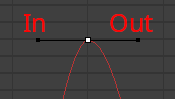
\includegraphics[width=0.4\textwidth]{imagenes/4-2.png}
    \caption{Puntos de control del fotograma clave.}
\end{figure}

De estos pares de valores, el de arriba modifica la posición en el eje Y (vertical) del punto de control y el de abajo modifica la longitud desde el fotograma clave hasta el punto de control.

\section{¿Por qué puede ser tan importante considerar el sistema de referencia en una animación?}
Porque es la base para definir como se mueven los objetos en el espacio. Utilizando un sistema de referencia se pueden realizar animaciones coherentes y realistas, ya que si no se usa puede parecer que la animación no es correcta o que incluso no hay animación.
\subsection{Da un ejemplo en el que la animación varíe dependiendo del sistema de referencia.}
Un ejemplo es el típico que se explica en lecciones de física: El observador dentro de un tren en movimiento ve que el exterior se está moviendo y él está parado. Mientras que un observador en el exterior ve el tren en movimiento y el paisaje parado \cite{explicacion}.

\bigskip

Otro ejemplo más cercano a las animaciones es el de una pelota que rebota. Un observador que se encuentra mirando directamente a esta pelota la ve rebotando de manera natural, mientras que otro que siga el movimiento de la pelota la verá parada y el resto de objetos en movimiento.

\section{Busca cuál es el problema que tiene la representación de rotaciones Gimbal.}

Antes de nada, un gimbal (cardán en español) es un conjunto de dos o tres aros concéntricos unidos por un eje al aro inmediatamente más grande. El gimbal permite mantener la orientación de un objeto con independencia de la rotación exterior \cite{eswiki:131649196}.

El bloqueo del gimbal consiste en la pérdida de un grado de libertad cuando dos de los tres aros se colocan en paralelo, bloqueando un eje de rotación en lo que se denomina un espacio bidimensional degenerado \cite{eswiki:119169170}.

\subsection{Provoca dicho problema en 3DS MAX.}

Para provocar dicho problema, lo primero que hay que hacer es cambiar el sistema de referencia en 3DS MAX. Para ello, hay que irse al menú desplegable de arriba y seleccionar la opción \textit{Gimbal} \cite{explicacion}.

\begin{figure}[H]
    \centering
    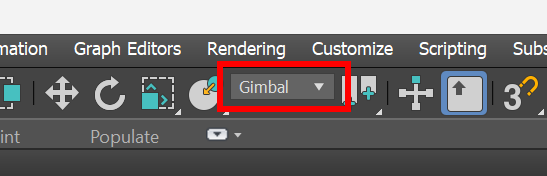
\includegraphics[width=0.8\textwidth]{imagenes/6-1.png}
    \caption{Sistema de referencia puesto en \textit{Gimbal}.}
\end{figure}

Una vez hecho esto, solo es necesario crear una figura y girarla 90 grados en el eje Y.

\begin{figure}[H]
    \centering
    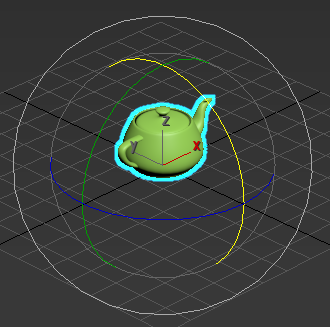
\includegraphics[width=0.6\textwidth]{imagenes/6-2.png}
    \caption{Tetera sin ninguna rotación, se puede ver que tiene los 3 ejes correctamente.}
\end{figure}

% foto de la tetera girada 90 grados
\begin{figure}[H]
    \centering
    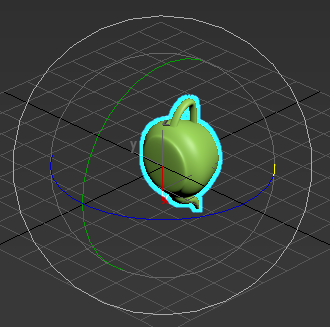
\includegraphics[width=0.6\textwidth]{imagenes/6-3.png}
    \caption{Tetera girada 90 grados en el eje Y, como se puede ver en la esfera de rotación, se han solapado dos ejes.}
\end{figure}

Ahora en este caso, la rotación en el eje X y en el eje Z provocan el mismo movimiento, habiendo perdido así un grado de libertad. Para arreglar esto, solo es necesario rotar de nuevo el eje Y a un valor distinto de 90 grados.

\newpage
\section{Crea un script sencillo en 3DS Max donde se usen los quaternions para girar un objeto 30º en uno de los ejes.}

Para ello, lo primero que hay que hacer es crear un nuevo proyecto y colocar una figura en la escena, en mi caso he puesto un cubo.

\begin{figure}[H]
    \centering
    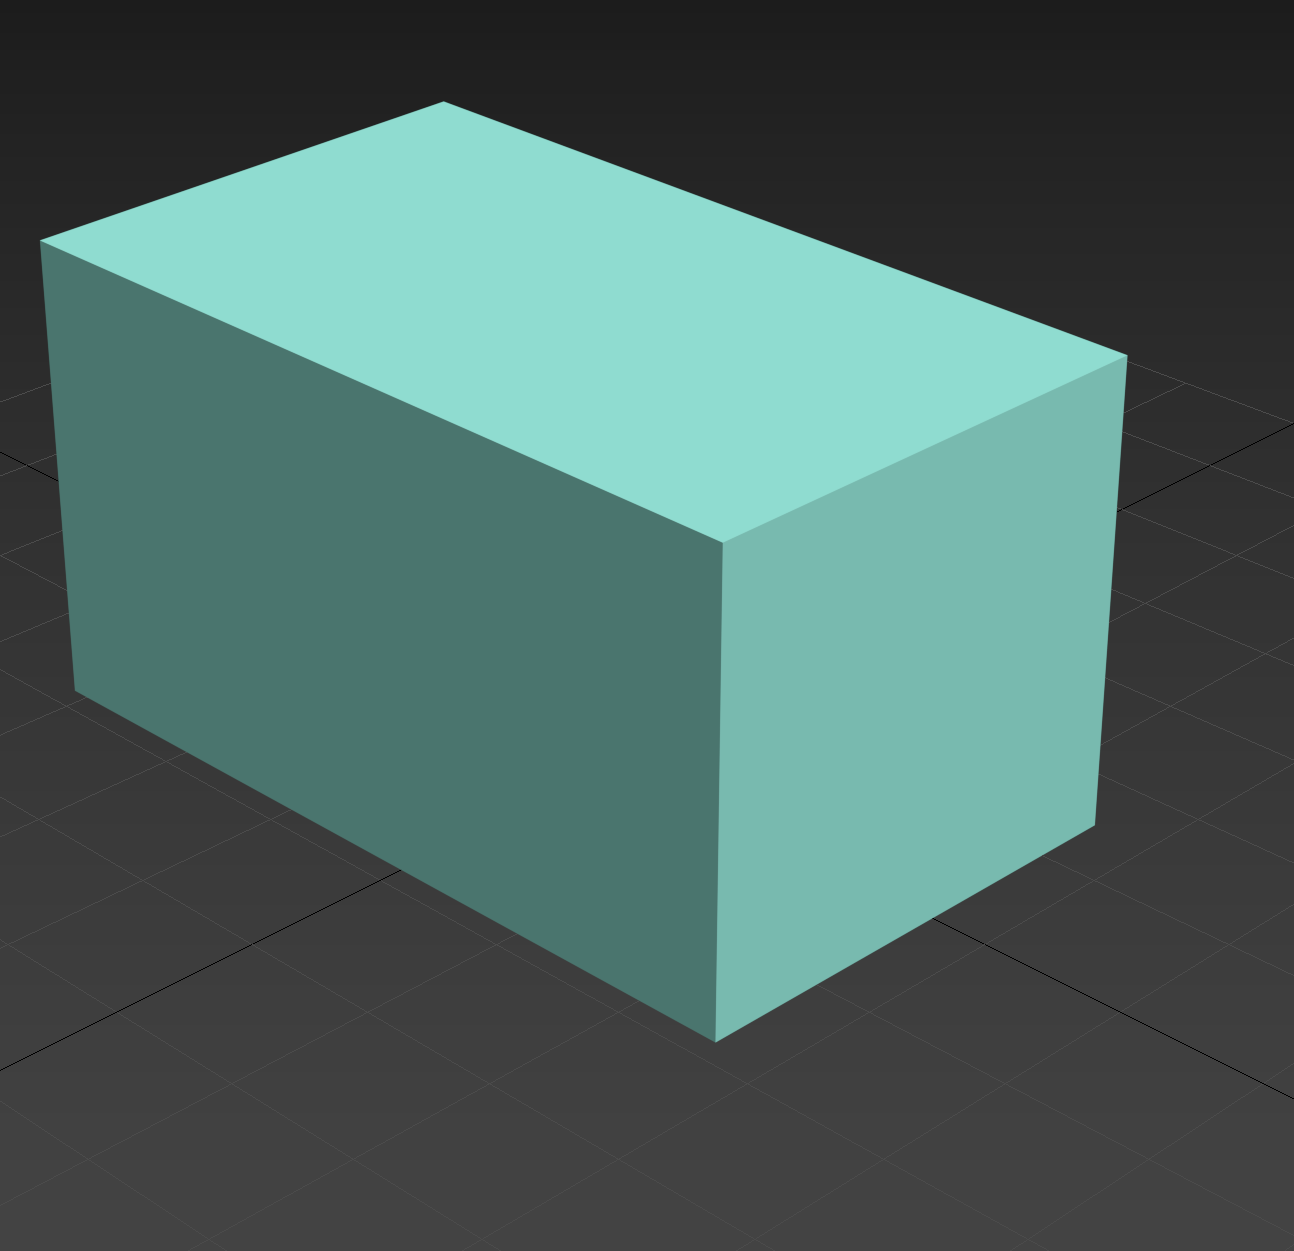
\includegraphics[width=0.6\textwidth]{imagenes/7-1.png}
    \caption{Escena inicial con el cubo creado.}
\end{figure}

Después hay que irse a los menús \textit{Scripting} $\rightarrow$ \textit{New file}. Y en el archivo hay que poner lo siguiente \cite{explicacion}:

% code snippet
\lstinputlisting[language=MaxScript]{rotate.ms}

Como se puede ver, solo se debe poner uno de los dos \verb|rotate|, el otro está comentado.

\bigskip

Y si abrimos el \textit{Scripting Listener}, y ejecutamos el script vemos lo siguiente:

% foto salida
\begin{figure}[H]
    \centering
    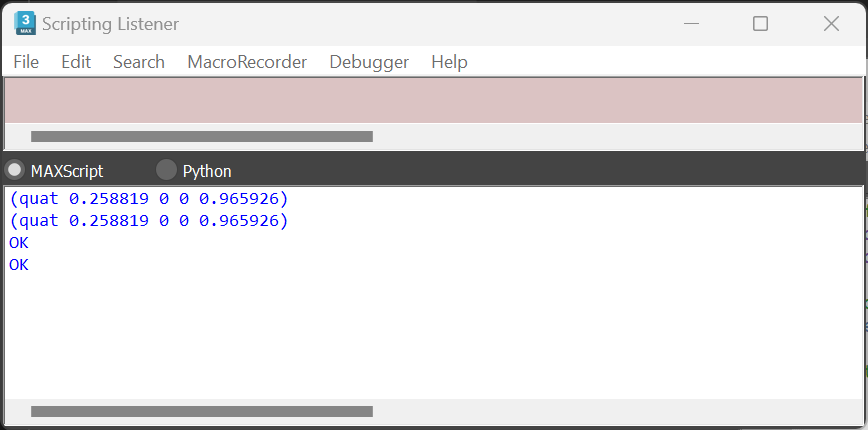
\includegraphics[width=0.7\textwidth]{imagenes/7-2.png}
    \caption{Vector resultante de hacer el quaternion de 30 grados en el eje X.}
\end{figure}

Que se corresponde a la fórmula de las transparencias, pero en otro orden. Además, se puede ver que ha salido dos veces, esto es debido a que se ha definido \verb|q1| y \verb|q2|.

\bigskip

Asimismo, el cubo de la escena se ha rotado 30 grados en el eje X:

\begin{figure}[H]
    \centering
    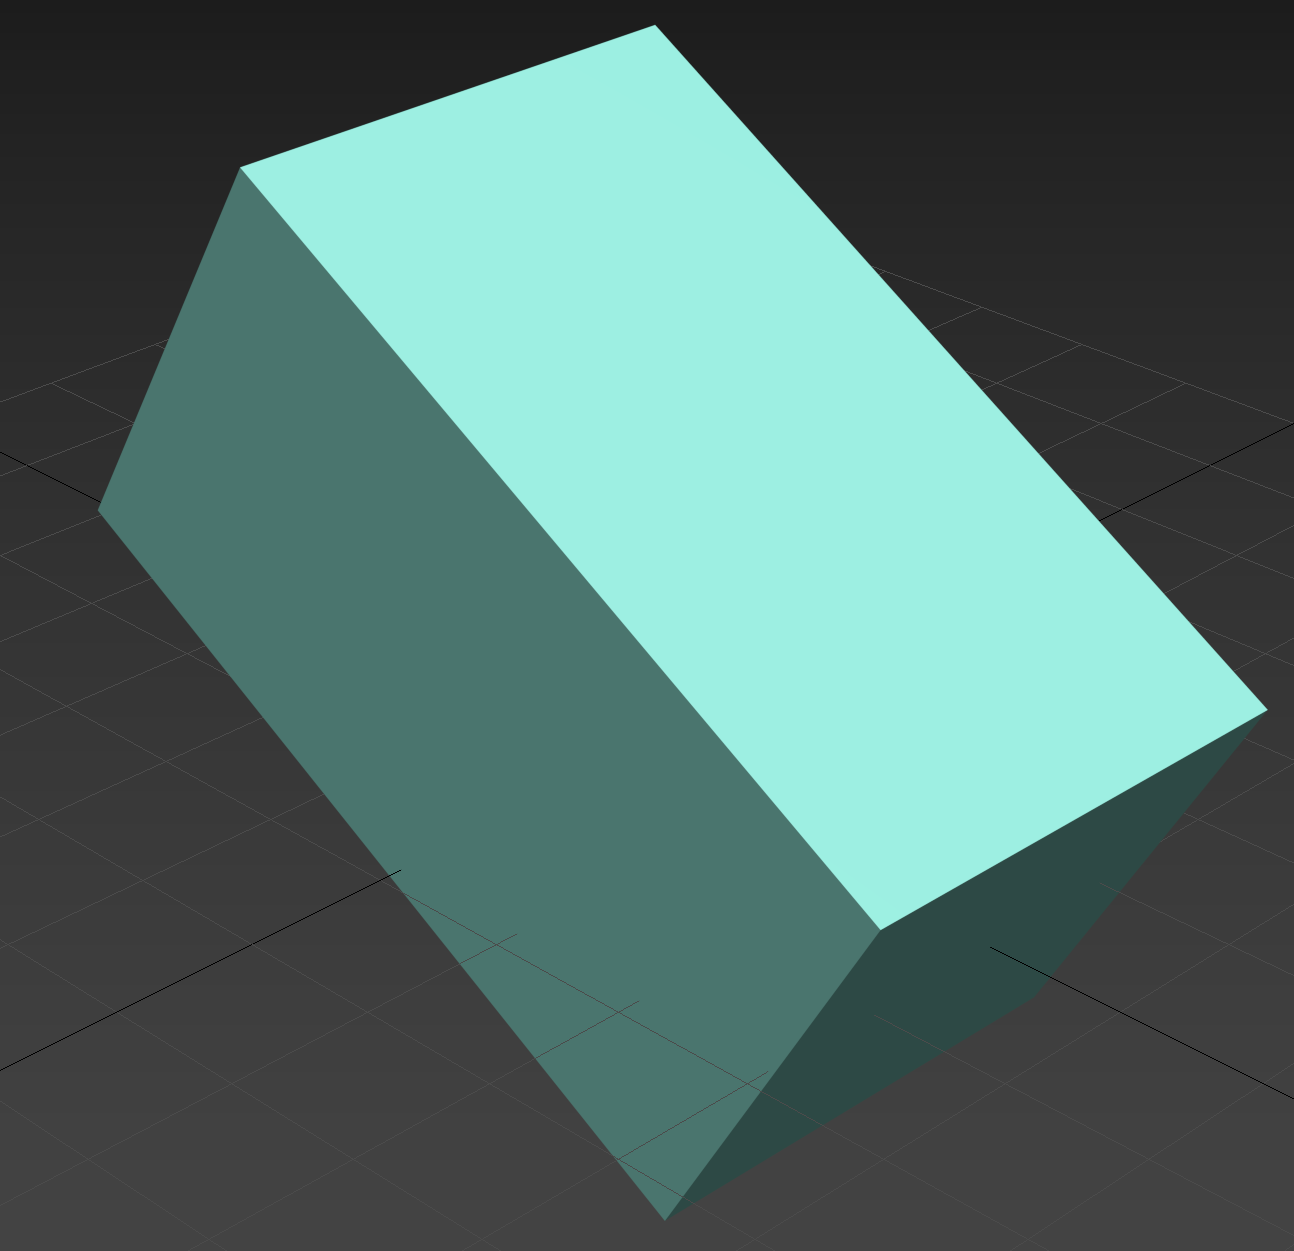
\includegraphics[width=0.6\textwidth]{imagenes/7-3.png}
    \caption{Cubo rotado mediante el script anterior.}
\end{figure}

\newpage

\bibliography{bibliografia}
\bibliographystyle{plainurl}
\end{document}
